\subsection{\boldmath$\sigma=5$ and a Second-order Neighborhood}
The first image sampled from the conditional posterior distribution $\mathbf{x}^{(1)}$ is shown in Figure \ref{fig:5d21} and the last image sampled from the conditional posterior distribution $\mathbf{x}^{(100)}$ is shown in Figure \ref{fig:5d2100}. 
The data image (in this case is also $\mathbf{x}^{(0)}$) and mean image are shown in Figure \ref{fig:ximage1} and Figure \ref{fig:5d2mean}.

We can see that all the images have the X shape as is in the data image.
However, $\mathbf{x}^{(1)}$, $\mathbf{x}^{(100)}$ did not recover all the information from the data image. 
For example, the pixel (19, 17) in the data image has a big value, making the pixel dark, but neither $\mathbf{x}^{(1)}$ nor $\mathbf{x}^{(100)}$ has a big value at pixel (19, 17). 
All $\mathbf{x}^{(1)}$, $\mathbf{x}^{(100)}$ and mean image have less contrast than the data image. 
The mean image is smoother than $\mathbf{x}^{(1)}$ and $\mathbf{x}^{(100)}$, since it averages all the 100 iterated images.
   \begin{figure*}[h]
        \centering
        \begin{subfigure}[b]{0.24\textwidth}
            \centering
            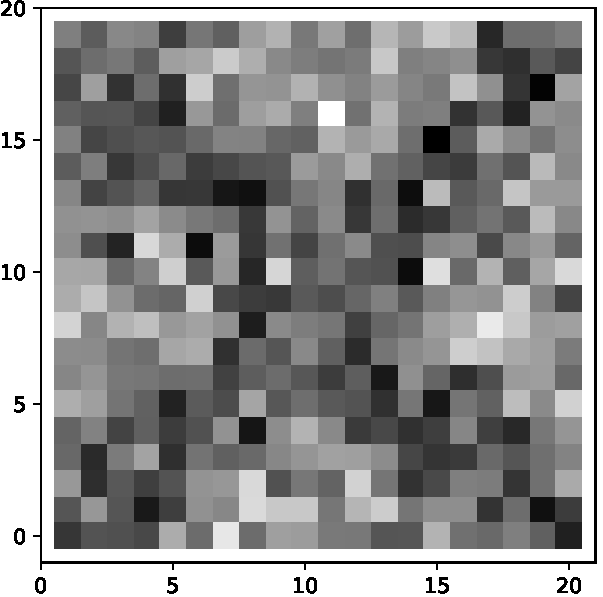
\includegraphics[width=\textwidth]{./img/ximage.pdf}
            \caption[]%
            {{\small $\mathbf{x}^{(0)}$}}    
            \label{fig:ximage1}
        \end{subfigure}
        \begin{subfigure}[b]{0.24\textwidth}  
            \centering 
            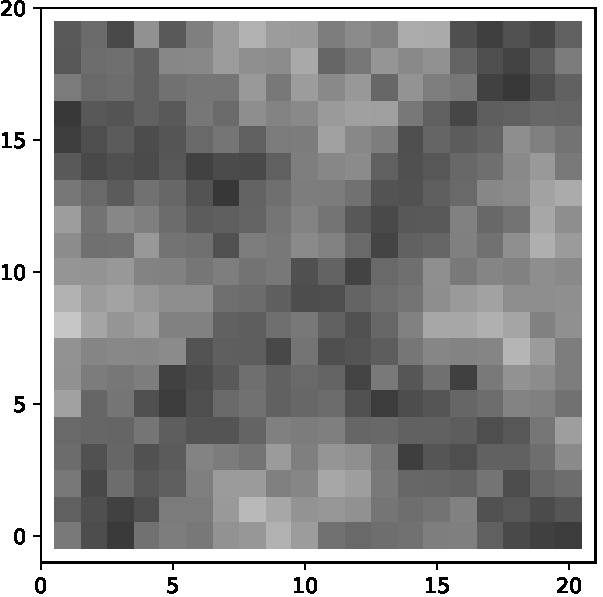
\includegraphics[width=\textwidth]{./img/5d2-0.pdf}
            \caption[]%
            {{\small $\mathbf{x}^{(1)}$}}    
            \label{fig:5d21}
        \end{subfigure}
        \begin{subfigure}[b]{0.24\textwidth}   
            \centering 
            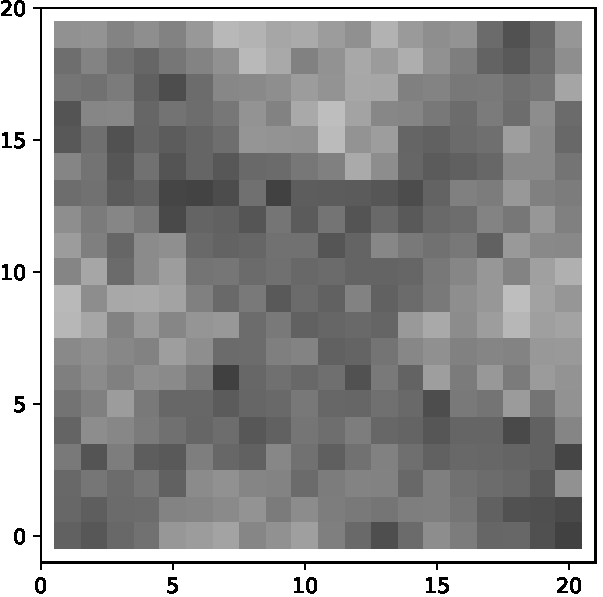
\includegraphics[width=\textwidth]{./img/5d2-99.pdf}
            \caption[]%
            {{\small $\mathbf{x}^{(100)}$}}    
            \label{fig:5d2100}
        \end{subfigure}
        \begin{subfigure}[b]{0.24\textwidth}   
            \centering 
            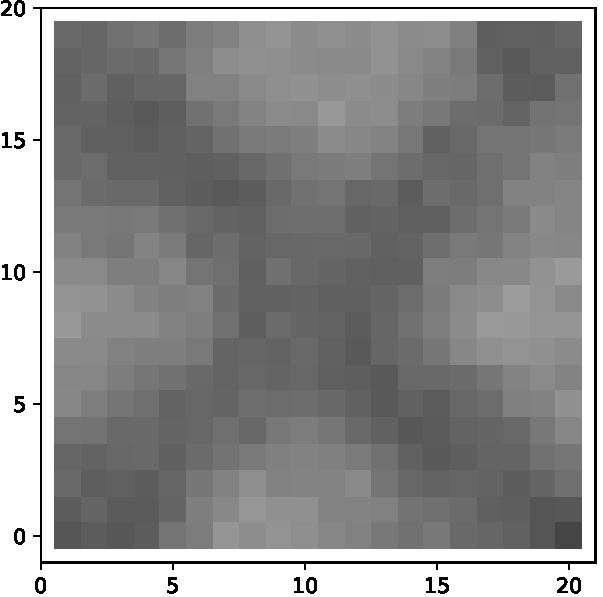
\includegraphics[width=\textwidth]{./img/5d2mean.pdf}
            \caption[]%
            {{\small Mean Image}}    
            \label{fig:5d2mean}
        \end{subfigure}
        \caption[]
        {\small Images obtained from a Gibbs sampler ($\sigma=5$ and a second-order neighborhood), with $\mathbf{x}^{(0)}$ as the observed data image, $\mathbf{x}^{(1)}$, and $\mathbf{x}^{(100)}$ as result from the first and last iteration. }
        \label{fig:5d2}
    \end{figure*}
\subsection{2 $\times$ 3 Factorial Design}
A 2 $\times$ 3 factorial design was conducted to compare the performance of various Gibbs samplers with different neighborhood order and $\sigma$ (Table \ref{factorial}). 
The illustration of neighborhood structures is shown in Figure \ref{fig:neiborill}.
\begin{table}[h]
\centering
\caption{2 $\times$ 3 Factorial Design}
\label{factorial}
\begin{tabular}{|l|l|l|l|}
\hline
                                                                                                & \multicolumn{3}{c|}{\begin{tabular}[c]{@{}c@{}}Factor B\\ $\sigma$\end{tabular}}                                                                                                                                                               \\ \hline
\multicolumn{1}{|c|}{\begin{tabular}[c]{@{}c@{}}Factor A\\ Neighborhood structure\end{tabular}} & \multicolumn{1}{c|}{\begin{tabular}[c]{@{}c@{}}j = 1\\ $\sigma=2$\end{tabular}} & \multicolumn{1}{c|}{\begin{tabular}[c]{@{}c@{}}j = 2\\ $\sigma=5$\end{tabular}} & \multicolumn{1}{c|}{\begin{tabular}[c]{@{}c@{}}j = 3\\ $\sigma=15$\end{tabular}} \\ \hline
i = 1 first-order                                                                               & Figure \ref{fig:2d1}                                                                          & Figure \ref{fig:5d1}                                                                          & Figure \ref{fig:15d1}                                                                            \\ \hline
i = 2 second-order                                                                              & Figure \ref{fig:2d2}                                                                           & Figure \ref{fig:5d2}                                                                           & Figure \ref{fig:15d2}                                                                            \\ \hline
\end{tabular}
\end{table}
\begin{figure}[h]
    \centering
    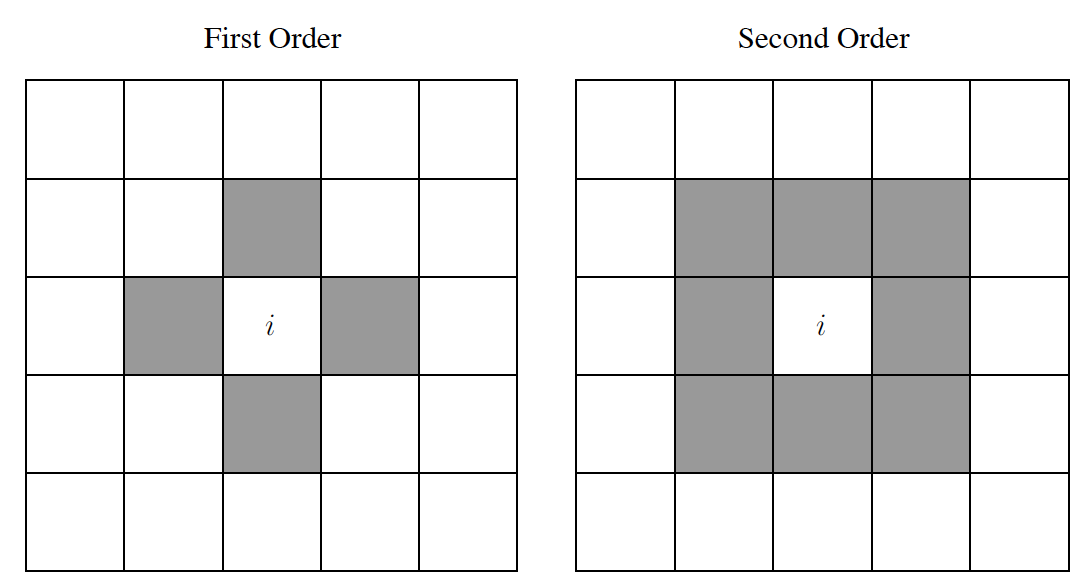
\includegraphics[scale=0.5]{./img/orderillus.png}
    \caption{Shaded pixels show a first-order (left) and a second-order neighborhood (right) in a rectangular lattice. (Figure adapted from text book \textbf{FIGURE 8.6} \cite{Givens}).}
    \label{fig:neiborill}
\end{figure}
\subsubsection{Factor: $\mathbf{\sigma}$}
First, we fix Factor A (neighborhood structure), and study how $\sigma$ effect the Gibbs sampler.
When we use the same neighborhood structure, we are fixing the conditional posterior distribution's mean, and the only thing changes is the variance of the conditional posterior normal distribution.
With larger $\sigma$, the Gibbs sampler samples larger width of a particular pixel's neighbors, meaning values of distant pixels can influence the sampled pixel. 

When first-order neighborhood is incorporated (Figure \ref{fig:2d1}, \ref{fig:5d1} and \ref{fig:15d1}), Figure \ref{fig:15d1} with $\sigma=15$ has a very steep gradient between pixels (high contrast), but has the least accurate shape of X because the distance pixels influence the sampled pixel. 
In contrast, images rendered from $\sigma=2$ have the least contrast among the three figures because the variance in conditional posterior distribution is small and Gibbs sampler depends more on the information from close neighborhoods. 
Figure \ref{fig:5d1} seems to be the best among these three figures. 

In the case of second-order neighborhood, Figure \ref{fig:15d2} has the highest contrast, while the images appear to be scrambled and X shape is totally lost. 
Figure \ref{fig:2d2} seems to be oversmoothed. Figure \ref{fig:5d2} seems to be the best among the three sets of images sampled from second-order neighborhood. 

\subsubsection{Factor: Neighborhood Structure}
Now, we investigate how the selection of neighborhood structure influence the images rendered by Gibbs sampler. 
Second-order neighborhood has 8 neighbors and first-order neighborhood only has 4 neighbors (Figure \ref{fig:neiborill}). 
The neighborhood structure influences both mean and variance of the conditional posterior distribution. 
The second-order neighborhood has smaller variance, while the value of mean depends on the data. 

The images below show that the images sampled from second-order neighborhood are smoother than those from first-order neighborhood. 
For example, images sampled from first-neighborhood (Figure \ref{fig:2d1}) seems to have higher contrast and are slightly better than the second-neighborhood (Figure \ref{fig:2d2}).
However, the differences between the images sampled using different neighborhood structures are not as large as those between images sampled using different $\sigma$'s.
%% 2d1 %%
   \begin{figure*}[!h]
        \centering
        \begin{subfigure}[b]{0.24\textwidth}
            \centering
            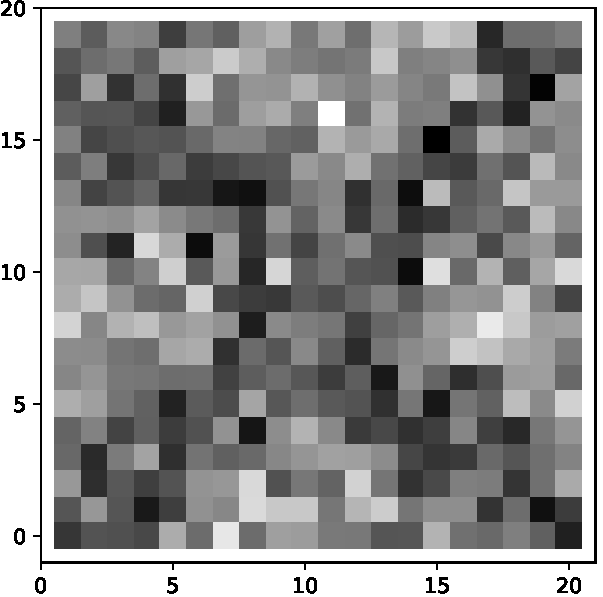
\includegraphics[width=\textwidth]{./img/ximage.pdf}
            \caption[]%
            {{\small $\mathbf{x}^{(0)}$}}    
            \label{fig:ximage2}
        \end{subfigure}
        \begin{subfigure}[b]{0.24\textwidth}  
            \centering 
            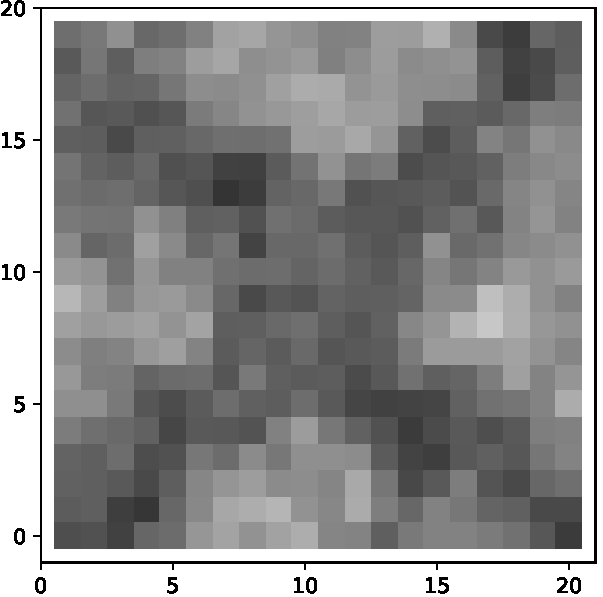
\includegraphics[width=\textwidth]{./img/2d1-0.pdf}
            \caption[]%
            {{\small $\mathbf{x}^{(1)}$}}    
            \label{fig:2d11}
        \end{subfigure}
        \begin{subfigure}[b]{0.24\textwidth}   
            \centering 
            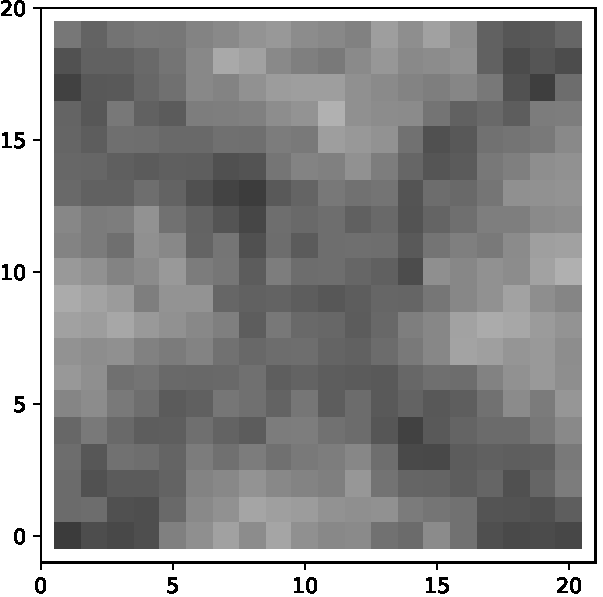
\includegraphics[width=\textwidth]{./img/2d1-99.pdf}
            \caption[]%
            {{\small $\mathbf{x}^{(100)}$}}    
            \label{fig:2d1100}
        \end{subfigure}
        \begin{subfigure}[b]{0.24\textwidth}   
            \centering 
            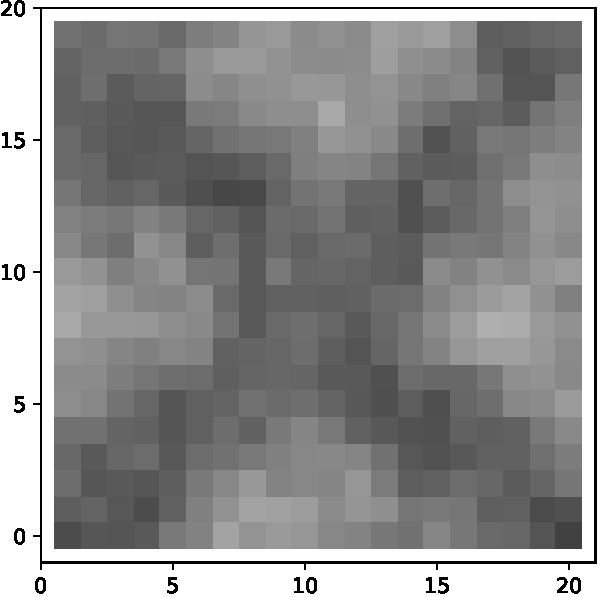
\includegraphics[width=\textwidth]{./img/2d1mean.pdf}
            \caption[]%
            {{\small Mean Image}}    
            \label{fig:2d1mean}
        \end{subfigure}
        \caption[]
        {\small Images obtained from a Gibbs sampler ($\sigma=2$ and a first-order neighborhood), with $\mathbf{x}^{(0)}$ as the observed data image, $\mathbf{x}^{(1)}$, and $\mathbf{x}^{(100)}$ as result from the first and last iteration. }
        \label{fig:2d1}
    \end{figure*}
%% 5d1 %%
   \begin{figure*}[!h]
        \centering
        \begin{subfigure}[b]{0.24\textwidth}
            \centering
            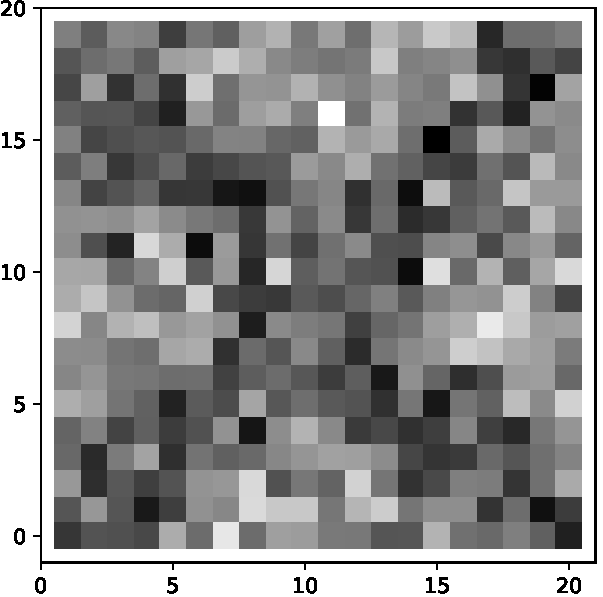
\includegraphics[width=\textwidth]{./img/ximage.pdf}
            \caption[]%
            {{\small $\mathbf{x}^{(0)}$}}    
            \label{fig:ximage3}
        \end{subfigure}
       % \hfill
        \begin{subfigure}[b]{0.24\textwidth}  
            \centering 
            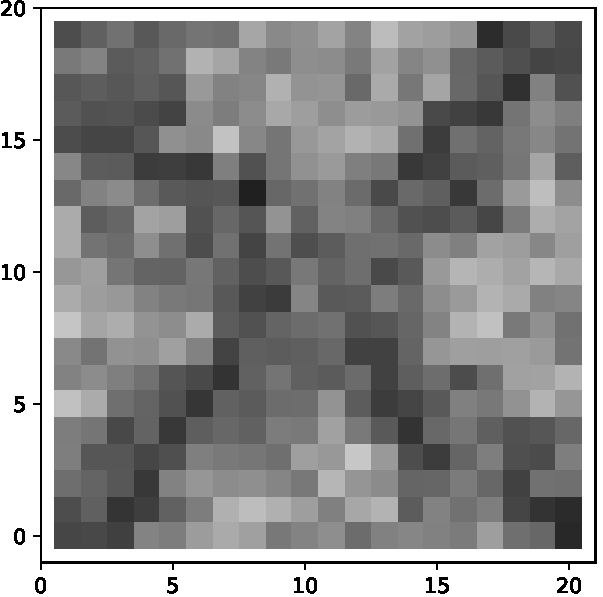
\includegraphics[width=\textwidth]{./img/5d1-0.pdf}
            \caption[]%
            {{\small $\mathbf{x}^{(1)}$}}    
            \label{fig:5d11}
        \end{subfigure}
       % \vskip\baselineskip
        \begin{subfigure}[b]{0.24\textwidth}   
            \centering 
            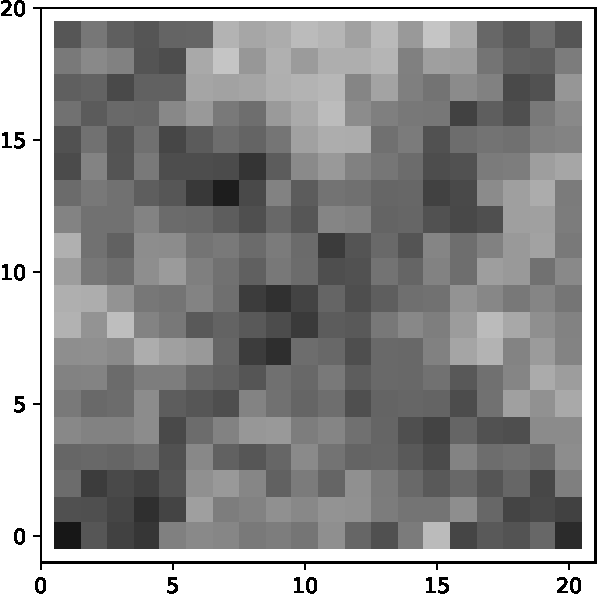
\includegraphics[width=\textwidth]{./img/5d1-99.pdf}
            \caption[]%
            {{\small $\mathbf{x}^{(100)}$}}    
            \label{fig:5d1100}
        \end{subfigure}
       % \quad
        \begin{subfigure}[b]{0.24\textwidth}   
            \centering 
            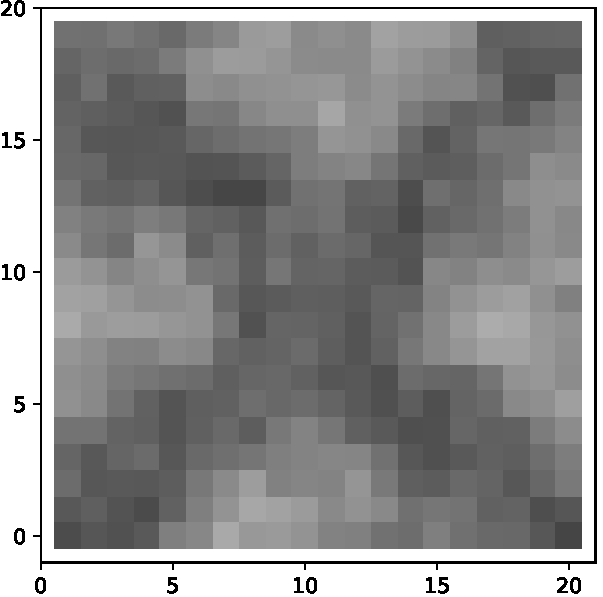
\includegraphics[width=\textwidth]{./img/5d1mean.pdf}
            \caption[]%
            {{\small Mean Image}}    
            \label{fig:5d1mean}
        \end{subfigure}
        \caption[]
        {\small Images obtained from a Gibbs sampler ($\sigma=5$ and a first-order neighborhood), with $\mathbf{x}^{(0)}$ as the observed data image, $\mathbf{x}^{(1)}$, and $\mathbf{x}^{(100)}$ as result from the first and last iteration.}
        \label{fig:5d1}
    \end{figure*}
%% 15d1 %%
   \begin{figure*}[!h]
        \centering
        \begin{subfigure}[b]{0.24\textwidth}
            \centering
            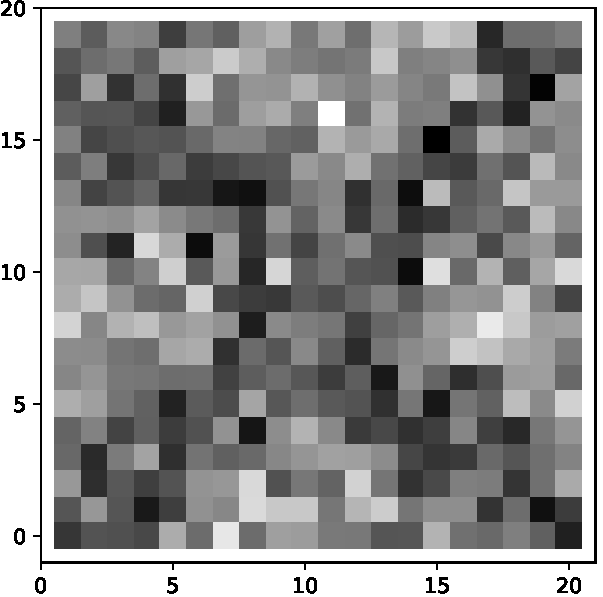
\includegraphics[width=\textwidth]{./img/ximage.pdf}
            \caption[]%
            {{\small $\mathbf{x}^{(0)}$}}    
            \label{fig:ximage4}
        \end{subfigure}
        %\hfill
        \begin{subfigure}[b]{0.24\textwidth}  
            \centering 
            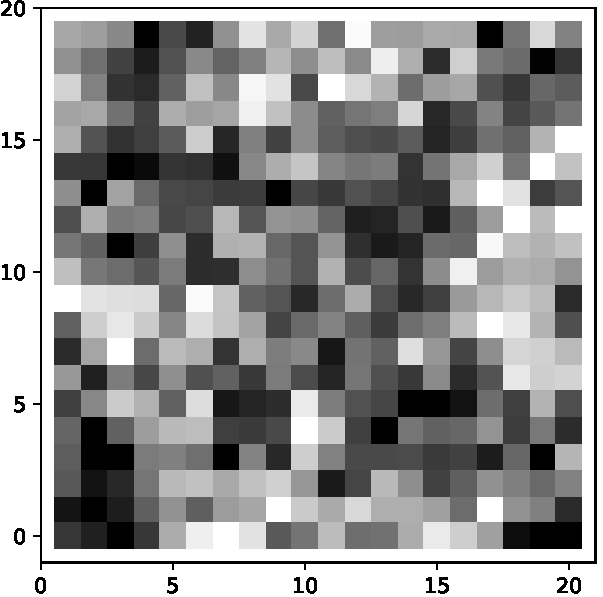
\includegraphics[width=\textwidth]{./img/15d1-0.pdf}
            \caption[]%
            {{\small $\mathbf{x}^{(1)}$}}    
            \label{fig:15d11}
        \end{subfigure}
       % \vskip\baselineskip
        \begin{subfigure}[b]{0.24\textwidth}   
            \centering 
            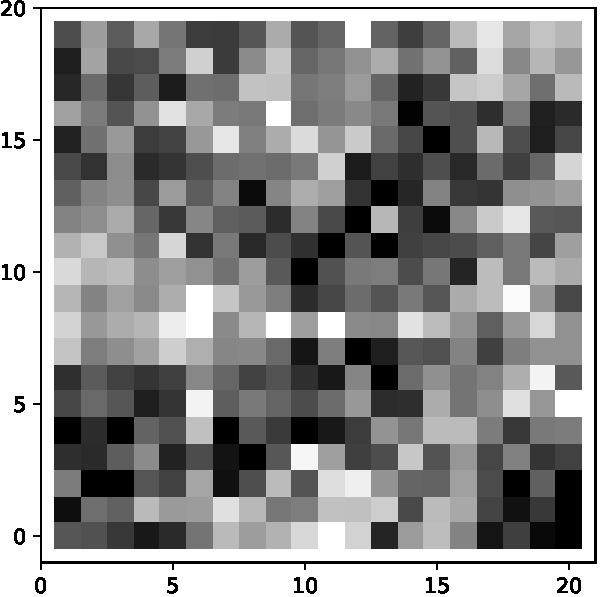
\includegraphics[width=\textwidth]{./img/15d1-99.pdf}
            \caption[]%
            {{\small $\mathbf{x}^{(100)}$}}    
            \label{fig:15d1100}
        \end{subfigure}
        %\quad
        \begin{subfigure}[b]{0.24\textwidth}   
            \centering 
            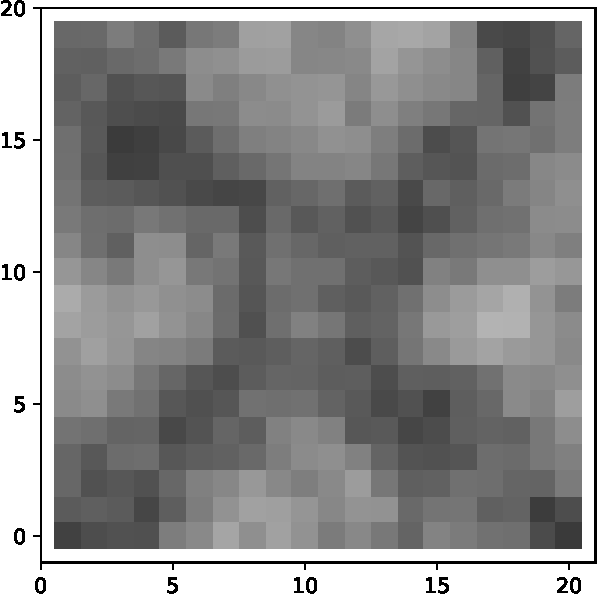
\includegraphics[width=\textwidth]{./img/15d1mean.pdf}
            \caption[]%
            {{\small Mean Image}}    
            \label{fig:15d1mean}
        \end{subfigure}
        \caption[]
        {\small Images obtained from a Gibbs sampler ($\sigma=15$ and a first-order neighborhood), with $\mathbf{x}^{(0)}$ as the observed data image, $\mathbf{x}^{(1)}$, and $\mathbf{x}^{(100)}$ as result from the first and last iteration. }
        \label{fig:15d1}
    \end{figure*}
%% 2d2 %%
   \begin{figure*}[!h]
        \centering
        \begin{subfigure}[b]{0.24\textwidth}
            \centering
            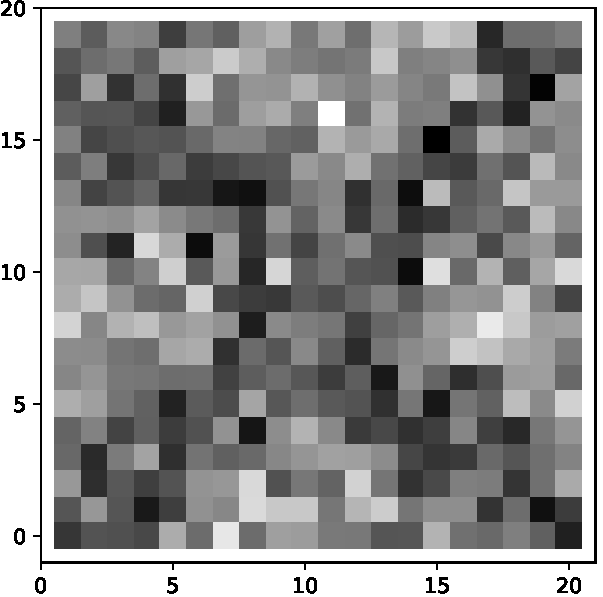
\includegraphics[width=\textwidth]{./img/ximage.pdf}
            \caption[]%
            {{\small $\mathbf{x}^{(0)}$}}    
            \label{fig:ximage5}
        \end{subfigure}
       % \hfill
        \begin{subfigure}[b]{0.24\textwidth}  
            \centering 
            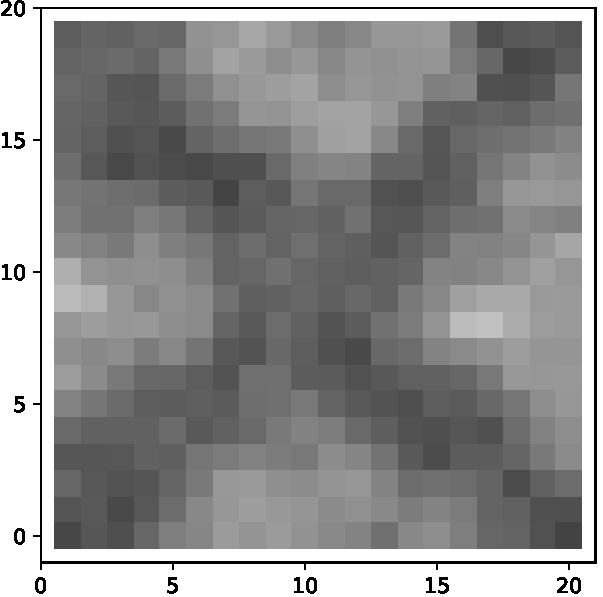
\includegraphics[width=\textwidth]{./img/2d2-0.pdf}
            \caption[]%
            {{\small $\mathbf{x}^{(1)}$}}    
            \label{fig:2d21}
        \end{subfigure}
        %\vskip\baselineskip
        \begin{subfigure}[b]{0.24\textwidth}   
            \centering 
            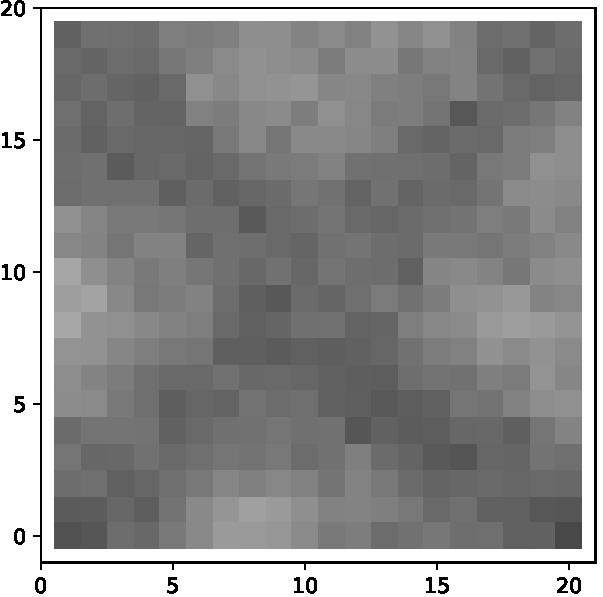
\includegraphics[width=\textwidth]{./img/2d2-99.pdf}
            \caption[]%
            {{\small $\mathbf{x}^{(100)}$}}    
            \label{fig:2d2100}
        \end{subfigure}
        %\quad
        \begin{subfigure}[b]{0.24\textwidth}   
            \centering 
            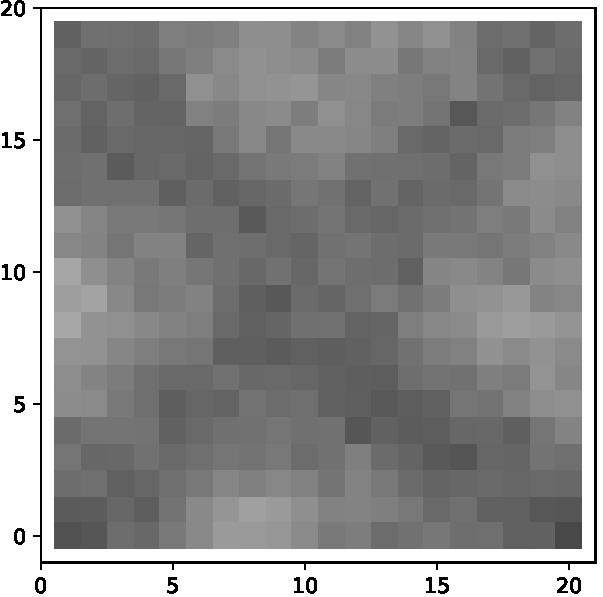
\includegraphics[width=\textwidth]{./img/2d2mean.pdf}
            \caption[]%
            {{\small Mean Image}}    
            \label{fig:2d2mean}
        \end{subfigure}
        \caption[]
        {\small Images obtained from a Gibbs sampler ($\sigma=2$ and a second-order neighborhood), with $\mathbf{x}^{(0)}$ as the observed data image, $\mathbf{x}^{(1)}$, and $\mathbf{x}^{(100)}$ as result from the first and last iteration. }
        \label{fig:2d2}
    \end{figure*}
%% 15d2 %%
   \begin{figure*}[!h]
        \centering
        \begin{subfigure}[b]{0.24\textwidth}
            \centering
            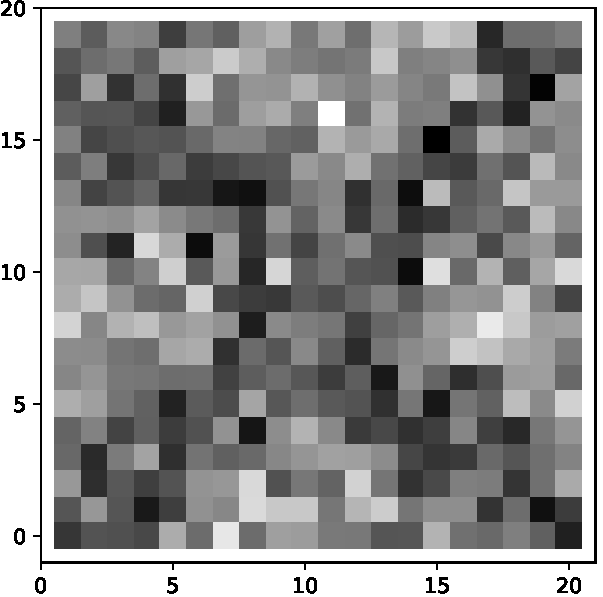
\includegraphics[width=\textwidth]{./img/ximage.pdf}
            \caption[]%
            {{\small $\mathbf{x}^{(0)}$}}    
            \label{fig:ximage6}
        \end{subfigure}
        %\hfill
        \begin{subfigure}[b]{0.24\textwidth}  
            \centering 
            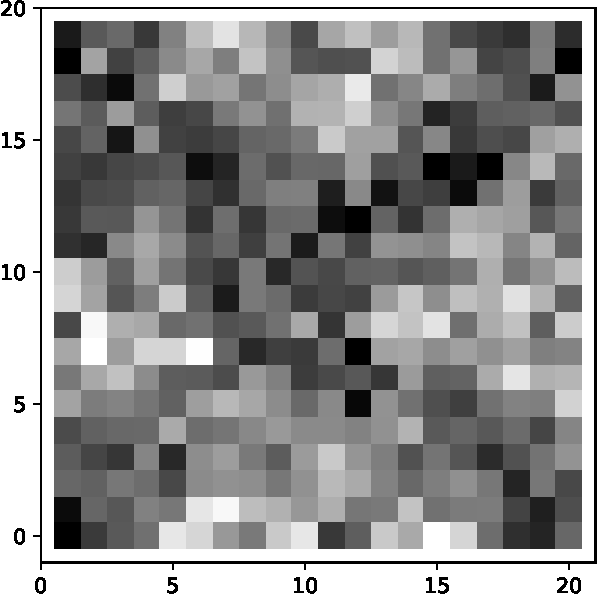
\includegraphics[width=\textwidth]{./img/15d2-0.pdf}
            \caption[]%
            {{\small $\mathbf{x}^{(1)}$}}    
            \label{fig:15d21}
        \end{subfigure}
        %\vskip\baselineskip
        \begin{subfigure}[b]{0.24\textwidth}   
            \centering 
            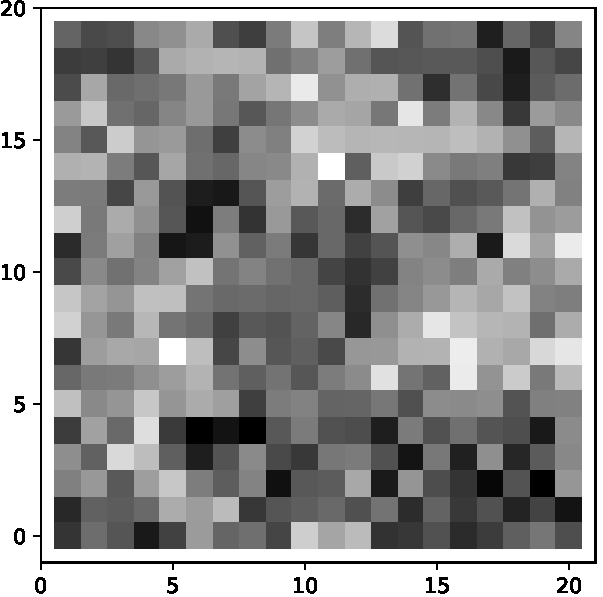
\includegraphics[width=\textwidth]{./img/15d2-99.pdf}
            \caption[]%
            {{\small $\mathbf{x}^{(100)}$}}    
            \label{fig:15d2100}
        \end{subfigure}
        %\quad
        \begin{subfigure}[b]{0.24\textwidth}   
            \centering 
            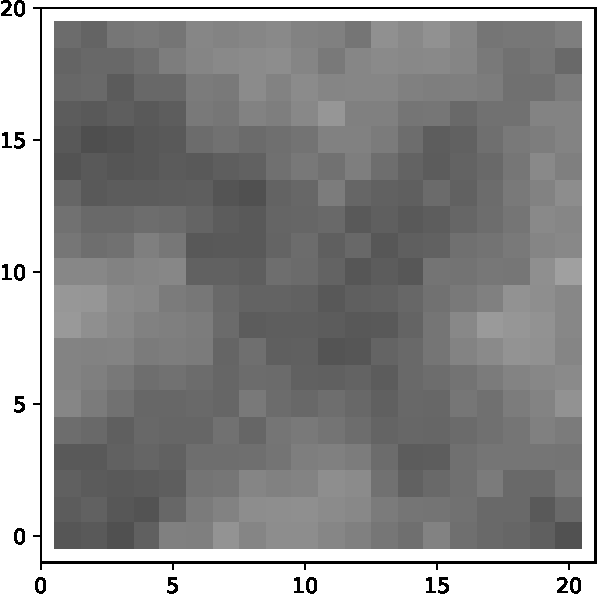
\includegraphics[width=\textwidth]{./img/15d2mean.pdf}
            \caption[]%
            {{\small Mean Image}}    
            \label{fig:15d2mean}
        \end{subfigure}
        \caption[]
        {\small Images obtained from a Gibbs sampler ($\sigma=15$ and a second-order neighborhood), with $\mathbf{x}^{(0)}$ as the observed data image, $\mathbf{x}^{(1)}$, and $\mathbf{x}^{(100)}$ as result from the first and last iteration. }
        \label{fig:15d2}
    \end{figure*}
\subsection{Different Starting $\mathbf{x^{(0)}}$}
$\mathbf{x}^{(0)}=57.5$, $\sigma=5$ and first-neighborhood were used for the Gibbs sampler. 
The result is shown in Figure \ref{fig:5755d1}. 
This Gibbs sampler uses the initial starting image $\mathbf{x}^{(0)}$ equal to the true posterior mean pixel color.
The results are pretty nice, neither too smooth, nor having too much contrast. 
The images are actually pretty close to those obtained by Gibbs sampler with $\mathbf{x}^{(0)}=$ the observed data image, $\sigma=5$ and a first-order neighborhood (Figure \ref{fig:5d1}). 
This indicates that the Markov chain moves fast from the initial state. 
Therefore, initial starting $\mathbf{x}^{(0)}$ is not very important in this case. 
%% 57.5 5d1 %%
   \begin{figure*}[!h]
        \centering
        \begin{subfigure}[b]{0.24\textwidth}
            \centering
            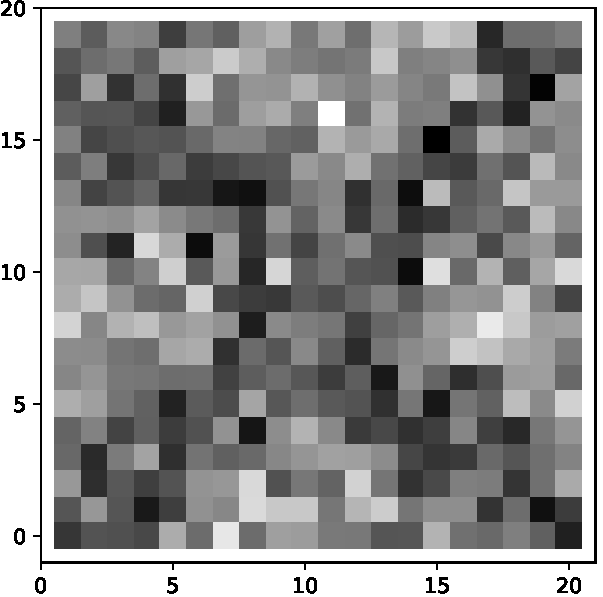
\includegraphics[width=\textwidth]{./img/ximage.pdf}
            \caption[]%
            {{\small Data Image}}    
            \label{fig:ximage7}
        \end{subfigure}
       % \hfill
        \begin{subfigure}[b]{0.24\textwidth}  
            \centering 
            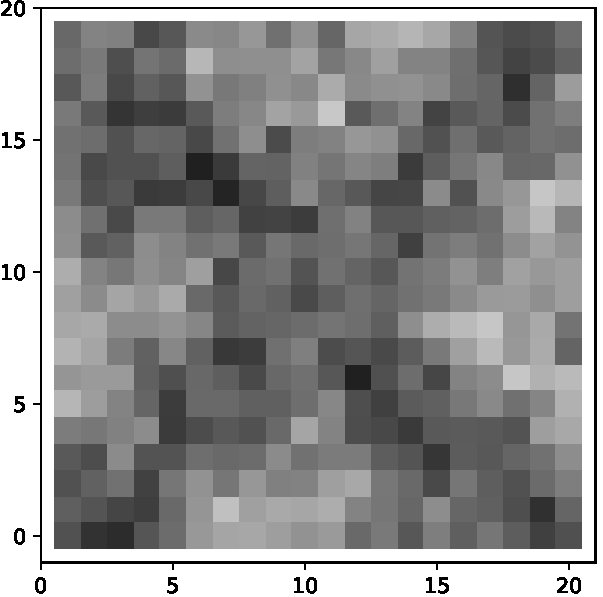
\includegraphics[width=\textwidth]{./img/5755d1-0.pdf}
            \caption[]%
            {{\small $\mathbf{x}^{(1)}$}}    
            \label{fig:57.55d11}
        \end{subfigure}
        %\vskip\baselineskip
        \begin{subfigure}[b]{0.24\textwidth}   
            \centering 
            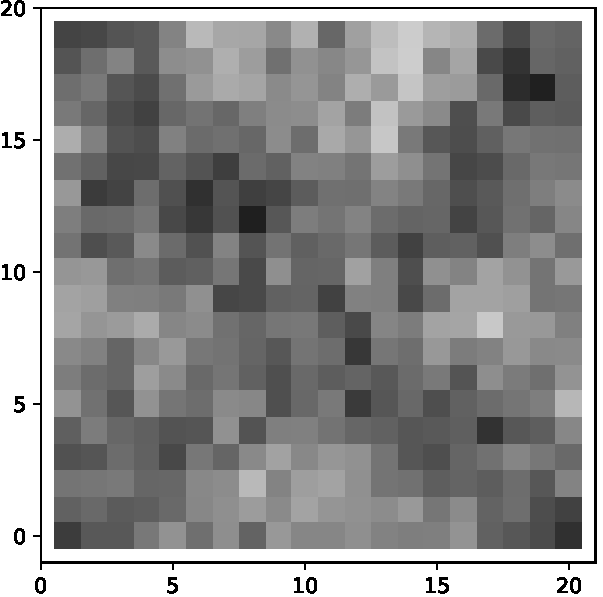
\includegraphics[width=\textwidth]{./img/5755d1-99.pdf}
            \caption[]%
            {{\small $\mathbf{x}^{(100)}$}}    
            \label{fig:57.55d1100}
        \end{subfigure}
       % \quad
        \begin{subfigure}[b]{0.24\textwidth}   
            \centering 
            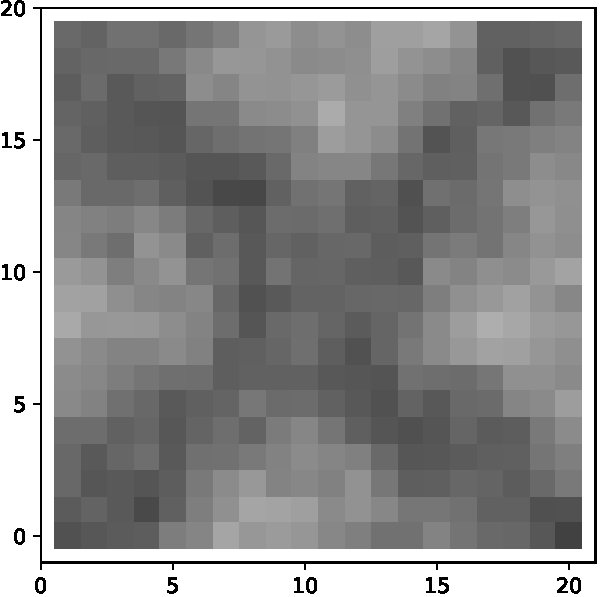
\includegraphics[width=\textwidth]{./img/5755d1mean.pdf}
            \caption[]%
            {{\small Mean Image}}    
            \label{fig:5755d1mean}
        \end{subfigure}
        \caption[]
        {\small Images obtained from a Gibbs sampler ($\sigma=5$ and a first-order neighborhood), with $\mathbf{x}^{(0)}=57.5$ as the observed data image, $\mathbf{x}^{(1)}$, and $\mathbf{x}^{(100)}$ as result from the first and last iteration. Note, (a) shows the data image that was observed, not the the initial starting image that was used for the Gibbs sampler. The presence of (a) here is just for comparison with images generated by the model in our project.}
        \label{fig:5755d1}
    \end{figure*}